\documentclass[tikz,border=16pt]{standalone}
\usepackage{amsmath,amssymb}
\usepackage{tikz}
\usetikzlibrary{arrows.meta, positioning, calc, fit, backgrounds, shapes.geometric}

%% ---- palette ----
\definecolor{cBlue}{RGB}{13,110,200}
\definecolor{cFillBlue}{RGB}{230,242,255}
\definecolor{cGray}{RGB}{95,108,120}
\definecolor{cFillGray}{RGB}{220,222,226}
\definecolor{cOrange}{RGB}{195,95,15}
\definecolor{cFillOrange}{RGB}{255,239,218}
\definecolor{cRed}{RGB}{170,35,35}
\definecolor{cFillRed}{RGB}{255,220,220}
\definecolor{cGreen}{RGB}{30,145,75}
\definecolor{cFillGreen}{RGB}{210,245,225}
\definecolor{cPurple}{RGB}{110,40,180}
\definecolor{cFillPurple}{RGB}{240,228,255}
\definecolor{cTeal}{RGB}{10,130,140}
\definecolor{cFillTeal}{RGB}{215,245,248}
\definecolor{cLegend}{RGB}{250,251,253}

\tikzset{
  actor/.style={rectangle, rounded corners=5pt, draw, minimum width=3.0cm,
                minimum height=0.8cm, font=\bfseries\small, align=center,
                inner sep=5pt, line width=1.4pt},
  actorV/.style={actor, draw=cBlue,   fill=cFillBlue,   text=cBlue},
  actorA/.style={actor, draw=cOrange, fill=cFillOrange, text=cOrange},
  %% computation boxes
  cbox/.style={rectangle, rounded corners=4pt, draw, minimum width=3.0cm,
               font=\scriptsize, align=left, inner sep=5pt, line width=1.1pt},
  cboxV/.style={cbox, draw=cBlue,   fill=cFillBlue,   text=cBlue},
  cboxA/.style={cbox, draw=cOrange, fill=cFillOrange, text=cOrange},
  cboxG/.style={cbox, draw=cGreen,  fill=cFillGreen,  text=cGreen},
  cboxT/.style={cbox, draw=cTeal,   fill=cFillTeal,   text=cTeal},
  %% abort box
  cboxR/.style={cbox, draw=cRed, fill=cFillRed, text=cRed},
  %% step bubble
  stepbubble/.style={circle, draw=cGray, fill=cFillGray, text=cGray,
                     font=\bfseries\scriptsize, inner sep=2pt, minimum size=0.5cm},
  %% arrows
  msgarrow/.style={-{Stealth[length=7pt]}, line width=1.4pt},
  msgarrowB/.style={msgarrow, draw=cBlue},
  msgarrowO/.style={msgarrow, draw=cOrange},
  msgarrowR/.style={msgarrow, draw=cRed, dashed},
  lifeline/.style={draw=cGray!40, line width=1pt, dashed},
  %% guard condition
  guard/.style={diamond, draw=cGray, fill=cFillGray, text=cGray,
                font=\bfseries\scriptsize, inner sep=2pt, align=center},
}

\begin{document}
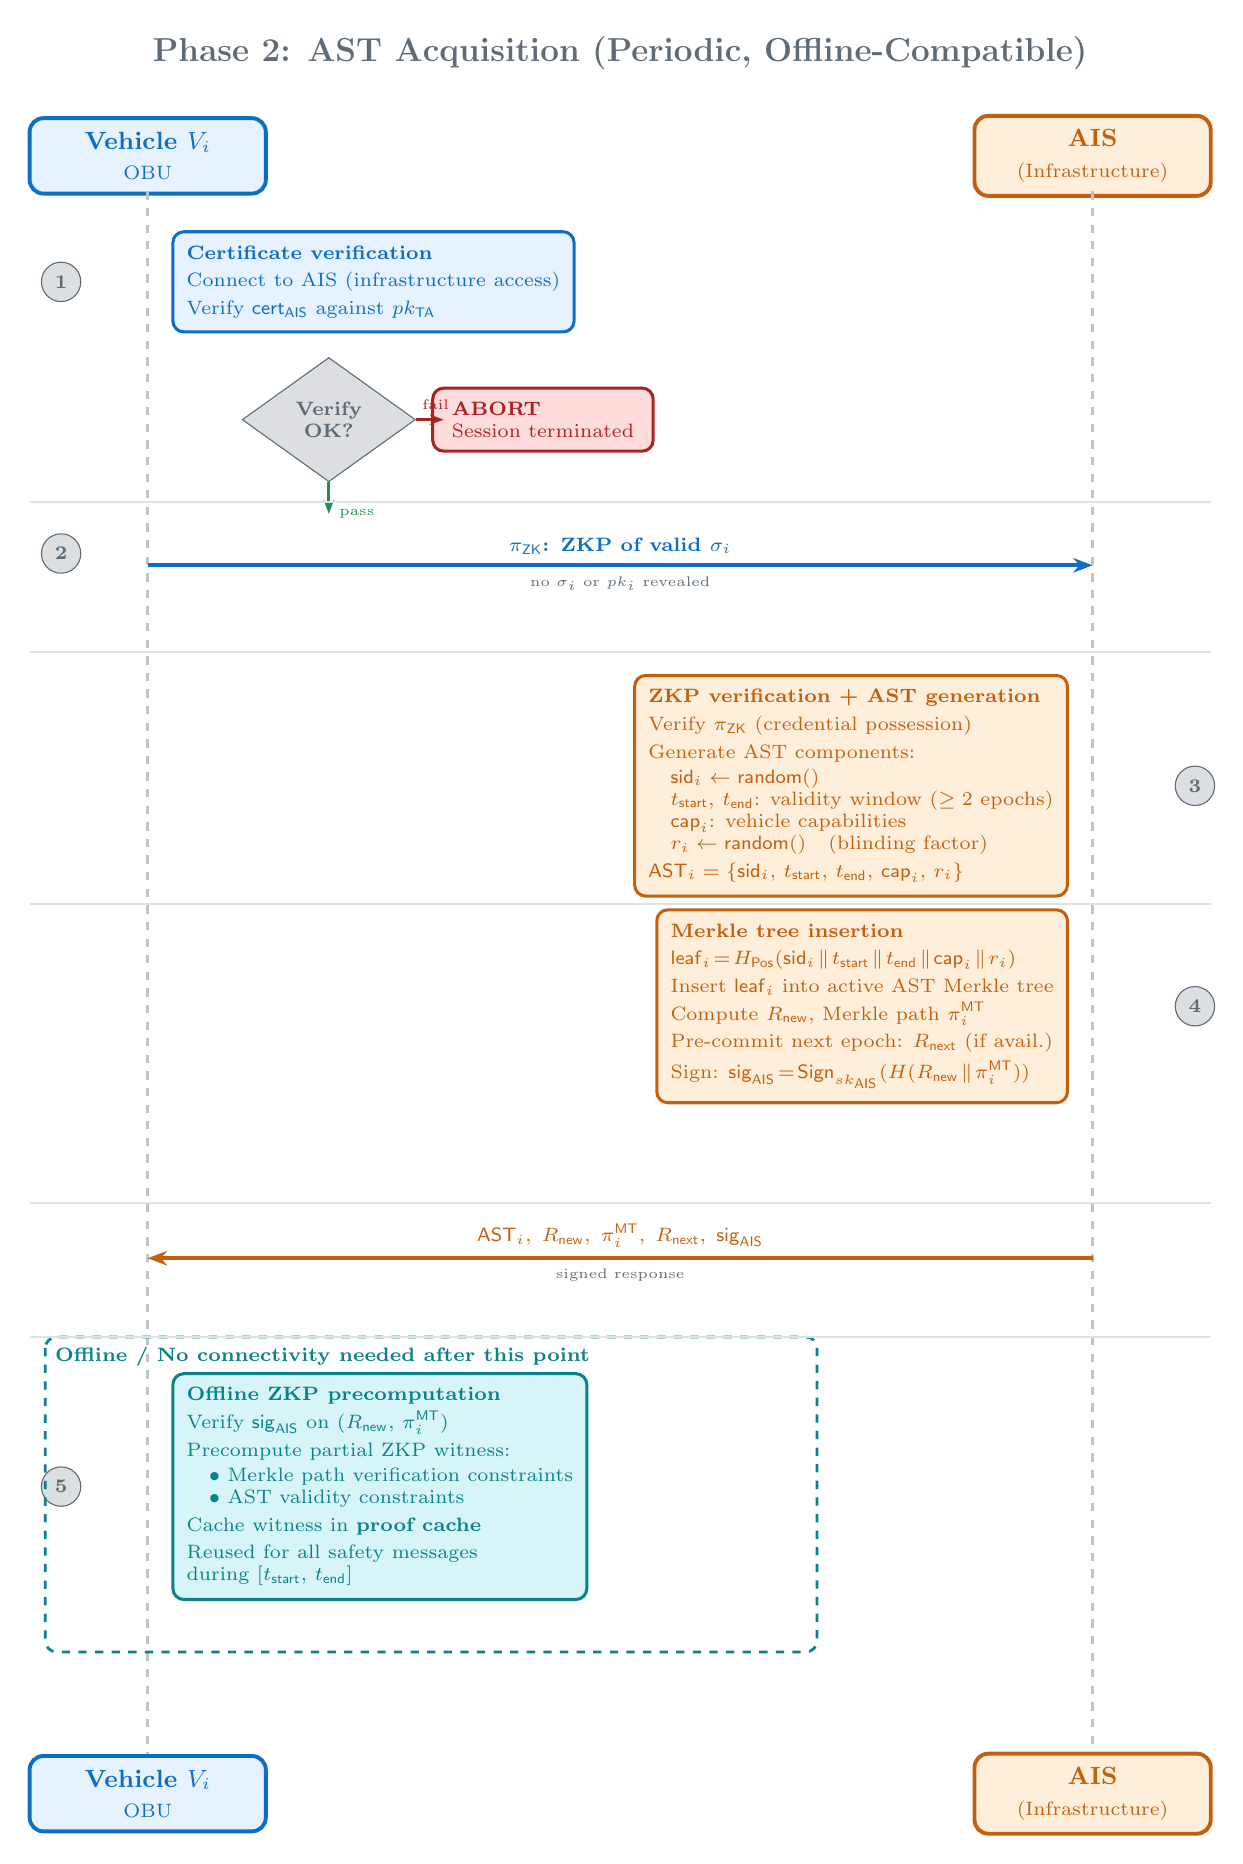
\begin{tikzpicture}

%% ============================================================
%%  ACTOR POSITIONS
%%  Vehicle Vi at x=0, AIS at x=12
%% ============================================================
\def\Vx{0}
\def\Ax{12}

%% ----- Actor headers -----
\node[actorV] (Vi)  at (\Vx,  0) {Vehicle $V_i$\\{\scriptsize\normalfont OBU}};
\node[actorA] (AIS) at (\Ax,  0) {AIS\\{\scriptsize\normalfont (Infrastructure)}};

%% ----- Lifelines -----
\draw[lifeline] (\Vx, -0.45) -- (\Vx, -20.8);
\draw[lifeline] (\Ax, -0.45) -- (\Ax, -20.8);

%% ============================================================
%%  STEP 1 — Connect + verify AIS cert  (y = -1.6)
%% ============================================================
\def\ya{-1.6}
\node[stepbubble] at (\Vx-1.1, \ya) {1};
\node[cboxV, anchor=west] at (\Vx+0.3, \ya) {%
  \textbf{Certificate verification}\\[2pt]
  Connect to AIS (infrastructure access)\\[2pt]
  Verify $\mathsf{cert}_{\mathsf{AIS}}$ against $pk_{\mathsf{TA}}$
};

%% guard diamond
\node[guard, minimum width=2.2cm, minimum height=0.65cm]
  (guard1) at (\Vx+2.3, -3.35) {Verify\\OK?};

%% fail branch
\node[cboxR, anchor=west, minimum width=2.8cm] at (\Vx+3.6, -3.35)
  {\textbf{ABORT}\\Session terminated};
\draw[-{Stealth[length=5pt]}, cRed, line width=1pt]
  (guard1.east) -- ++(0.35,0)
  node[above, font=\tiny, text=cRed, xshift=-0.1cm] {fail};

%% pass branch arrow down
\draw[-{Stealth[length=5pt]}, cGreen, line width=1pt]
  (guard1.south) -- ++(0,-0.4)
  node[right, font=\tiny, text=cGreen] {pass};

%% ============================================================
%%  STEP 2 — Vi sends ZKP of credential  (y = -5.2)
%% ============================================================
\def\yb{-5.2}
\node[stepbubble] at (\Vx-1.1, \yb+0.15) {2};

\draw[msgarrowB] (\Vx, \yb) -- (\Ax, \yb)
  node[midway, above, font=\scriptsize\bfseries, text=cBlue]
    {$\pi_{\mathsf{ZK}}$: ZKP of valid $\sigma_i$}
  node[midway, below, font=\tiny, text=cGray]
    {no $\sigma_i$ or $pk_i$ revealed};

%% ============================================================
%%  STEP 3 — AIS verifies ZKP + generates AST  (y = -7.0)
%% ============================================================
\def\yc{-8.0}
\node[stepbubble] at (\Ax+1.3, \yc) {3};
\node[cboxA, anchor=east] at (\Ax-0.3, \yc) {%
  \textbf{ZKP verification + AST generation}\\[2pt]
  Verify $\pi_{\mathsf{ZK}}$ (credential possession)\\[2pt]
  Generate AST components:\\[1pt]
  \quad $\mathsf{sid}_i \leftarrow \mathsf{random}()$\\
  \quad $t_{\mathsf{start}},\, t_{\mathsf{end}}$: validity window ($\geq 2$ epochs)\\
  \quad $\mathsf{cap}_i$: vehicle capabilities\\
  \quad $r_i \leftarrow \mathsf{random}()$\quad (blinding factor)\\[2pt]
  $\mathsf{AST}_i = \{\mathsf{sid}_i,\, t_{\mathsf{start}},\, t_{\mathsf{end}},\, \mathsf{cap}_i,\, r_i\}$
};

%% ============================================================
%%  STEP 4 — AIS computes leaf + Merkle update  (y = -10.8)
%% ============================================================
\def\yd{-10.8}
\node[stepbubble] at (\Ax+1.3, \yd) {4};
\node[cboxA, anchor=east] at (\Ax-0.3, \yd) {%
  \textbf{Merkle tree insertion}\\[2pt]
  $\mathsf{leaf}_i \!=\! H_{\mathsf{Pos}}(\mathsf{sid}_i \!\parallel\! t_{\mathsf{start}} \!\parallel\! t_{\mathsf{end}} \!\parallel\! \mathsf{cap}_i \!\parallel\! r_i)$\\[2pt]
  Insert $\mathsf{leaf}_i$ into active AST Merkle tree\\[2pt]
  Compute $R_{\mathsf{new}}$, Merkle path $\pi^{\mathsf{MT}}_i$\\[2pt]
  Pre-commit next epoch: $R_{\mathsf{next}}$ (if avail.)\\[2pt]
  Sign: $\mathsf{sig}_{\mathsf{AIS}} \!=\! \mathsf{Sign}_{sk_{\mathsf{AIS}}}(H(R_{\mathsf{new}} \!\parallel\! \pi^{\mathsf{MT}}_i))$
};

%% AIS -> Vi return arrow
\def\ye{-14.0}
\draw[msgarrowO] (\Ax, \ye) -- (\Vx, \ye)
  node[midway, above, font=\scriptsize\bfseries, text=cOrange]
    {$\mathsf{AST}_i,\; R_{\mathsf{new}},\; \pi^{\mathsf{MT}}_i,\; R_{\mathsf{next}},\; \mathsf{sig}_{\mathsf{AIS}}$}
  node[midway, below, font=\tiny, text=cGray]
    {signed response};

%% ============================================================
%%  STEP 5 — Offline Precomputation  (y = -15.6)
%% ============================================================
\def\yf{-16.9}
\node[stepbubble] at (\Vx-1.1, \yf) {5};
\node[cboxT, anchor=west] at (\Vx+0.3, \yf) {%
  \textbf{Offline ZKP precomputation}\\[2pt]
  Verify $\mathsf{sig}_{\mathsf{AIS}}$ on $(R_{\mathsf{new}},\, \pi^{\mathsf{MT}}_i)$\\[2pt]
  Precompute partial ZKP witness:\\[1pt]
  \quad $\bullet$~Merkle path verification constraints\\
  \quad $\bullet$~AST validity constraints\\[2pt]
  Cache witness in \textbf{proof cache}\\[2pt]
  Reused for all safety messages\\
  during $[t_{\mathsf{start}},\, t_{\mathsf{end}}]$
};

%% ============================================================
%%  "OFFLINE" annotation banner
%% ============================================================
\draw[cTeal, dashed, line width=1pt, rounded corners=4pt]
  (-1.3, -15.0) rectangle (8.5, -19.0);
\node[cTeal, font=\bfseries\scriptsize, anchor=north west]
  at (-1.3, -15.0) {Offline / No connectivity needed after this point};

%% ============================================================
%%  TITLE
%% ============================================================
\node[font=\bfseries\large, text=cGray] at (6, 1.3)
  {Phase 2: AST Acquisition (Periodic, Offline-Compatible)};

%% ============================================================
%%  Horizontal separators
%% ============================================================
\foreach \yy in {-4.4, -6.3, -9.5, -13.3, -15.0} {
  \draw[cGray!20, line width=0.7pt] (-1.5, \yy) -- (13.5, \yy);
}

%% ============================================================
%%  Actor footers
%% ============================================================
\node[actorV] at (\Vx,  -20.8) {Vehicle $V_i$\\{\scriptsize\normalfont OBU}};
\node[actorA] at (\Ax,  -20.8) {AIS\\{\scriptsize\normalfont (Infrastructure)}};

\end{tikzpicture}
\end{document}